% 编译: latexmk -xelatex paper_zh.tex
\documentclass[11pt,journal,onecolumn]{IEEEtran}
\usepackage{amsmath,amssymb,amsthm}
\usepackage{bm}
\usepackage{graphicx}
\usepackage{booktabs}
\usepackage{array}
\usepackage{cite}
\usepackage{algorithm}
\usepackage{algpseudocode}
\floatname{algorithm}{算法}
\renewcommand{\algorithmicrequire}{\textbf{输入:}}
\renewcommand{\algorithmicensure}{\textbf{输出:}}
\newcommand{\placeholderbox}[2]{\fbox{\parbox[c][#1][c]{0.9\linewidth}{\centering\textbf{【实验数据占位】}\\[3pt]#2}}}
\usepackage{fontspec}
\setmainfont{TeX Gyre Termes}
\makeatletter
\edef\@tmp{\noexpand\DeclareFontFamilySubstitution{TU}{ptm}{\rmdefault}}\@tmp
\makeatother
\usepackage{xeCJK}
\setCJKmainfont[
  Path={D:/texlive/2026/texmf-dist/fonts/opentype/public/fandol/},
  BoldFont={FandolSong-Bold.otf},
  ItalicFont={FandolKai-Regular.otf}
]{FandolSong-Regular.otf}
\setCJKsansfont[
  Path={D:/texlive/2026/texmf-dist/fonts/opentype/public/fandol/},
  BoldFont={FandolHei-Bold.otf}
]{FandolHei-Regular.otf}
\setCJKmonofont[
  Path={D:/texlive/2026/texmf-dist/fonts/opentype/public/fandol/}
]{FandolFang-Regular.otf}
\usepackage[colorlinks=false,pdfborder={0 0 0}]{hyperref}

\renewcommand{\abstractname}{摘\quad 要}
\renewcommand{\IEEEkeywordsname}{关键词}
\renewcommand{\figurename}{图}
\renewcommand{\tablename}{表}
\renewcommand{\appendixname}{附录}
\renewcommand{\refname}{参考文献}

\theoremstyle{plain}
\newtheorem{theorem}{定理}
\newtheorem{lemma}{引理}
\newtheorem{proposition}{命题}
\theoremstyle{remark}
\newtheorem{remark}{注}
\renewcommand{\proofname}{证明}

\newcommand{\zv}{\mathbf{z}}
\newcommand{\uv}{\mathbf{u}}
\newcommand{\bv}{\mathbf{b}}
\newcommand{\nv}{\mathbf{n}}
\newcommand{\tv}{\mathbf{t}}
\newcommand{\vv}{\mathbf{v}}
\newcommand{\phiv}{\bm{\varphi}}
\newcommand{\Jc}{\mathcal{J}}
\newcommand{\Lc}{\mathcal{L}}
\newcommand{\atan}{\operatorname{atan2}}
\newcommand{\T}{\mathsf{T}}

\begin{document}

\title{马赫--曾德尔调制器及其双平行结构\\任意点偏压控制的精确仿射框架}

\author{第一作者，第二作者%
\thanks{论文草稿。作者姓名、单位与基金信息待补充。作者单位：西安电子科技大学综合业务网理论及关键技术国家重点实验室，西安~710071。}}

\markboth{预印本 --- MZM/DPMZM 偏压控制的仿射框架}%
{作者~\MakeLowercase{\textit{等}}：任意点偏压控制的精确仿射框架}

\maketitle

\begin{abstract}
基于导频（dither）的马赫--曾德尔调制器（MZM）偏压控制器传统上只能锁定少数特殊工作点（正交点、零点、峰值点），其根源在于任何标量谐波误差信号在一个完整偏置周期内必然存在死区与分支歧义。本文建立一个\emph{精确}的结构定理：对任意周期导频波形与任意线性接收链，谐波解调观测向量是由偏置相位参数化的单位圆~$\mathbb{S}^1$ 的仿射像；增益失配、参考相位误差、导频波形失真、相干串扰、有限消光比等一切线性非理想因素只改变仿射参数~$(A,\bv)$ 的取值，而永远不改变模型的形式。由此，任意点偏压控制化归为椭圆辨识加直接~$\atan$ 相位解调——结构上即移植到偏压域、并与控制律联立的~Heydemann 校正——所得控制回路的增益在整个偏置周期上一致，所有传统方案的静态锁定误差亦以仿射元素比值的闭式统一给出。框架进而精确推广至双平行~MZM（DPMZM）：状态流形升为三维环面~$\mathbb{T}^3$，仿射性由一个含半角项的~12 维三角特征映射保持。半角结构蕴含子轴~$4\pi$ 标定周期与~Klein 四元群构型等价，并导出一条最具工程后果的可观测性定理：六个谐波通道的奇异集恰为标准~QPSK 工作点的~Klein 轨道，故文献中以互调（IMD）音检测父偏置的做法是秩条件的必然要求而非工程巧思。相应地，标定推广为单条准周期空间填充扫描上的线性回归，解调推广为热启动高斯--牛顿迭代，每控制周期代价低于~$10^3$ 次乘加。数值验证表明：零噪声极限下全链路闭合达机器精度；真实噪声下解调残差为毫弧度量级；任意目标点处较传统多环锁定改善一至两个数量级，后者在该场景下呈现数百毫弧度的静差乃至完全失锁。
\end{abstract}

\begin{IEEEkeywords}
马赫--曾德尔调制器，双平行~MZM，偏压控制，导频，仿射辨识，椭圆拟合，可观测性，高斯--牛顿，微波光子学。
\end{IEEEkeywords}

\IEEEpeerreviewmaketitle
\setlength{\emergencystretch}{2em}

\section{引言}
铌酸锂（LiNbO$_3$）与磷化铟（InP）马赫--曾德尔调制器（MZM）受温度、电荷积累与光折变效应影响而产生缓慢的偏置漂移~\cite{salvestrini2011,chen2011}，这一问题同样延续到新兴的薄膜铌酸锂平台~\cite{wang2018,wang2022}。基于小幅低频导频（dither）的闭环偏压控制是事实上的标准：探测光电流的一、二次谐波分别在零/峰值点与正交点处过零，构成误差信号；数十年的工程积累已使开关键控（OOK）的特殊点锁定以及面向~IQ 与偏振复用发射机的多环扩展相当成熟~\cite{cho2006,sotoodeh2011,kawakami2012,fu2013,li2017}。

然而，越来越多的应用要求把偏置停驻在\emph{任意}相位：微波光子移相器与矢量调制器~\cite{yao2009,capmany2007}、单边带（SSB）权重控制~\cite{izutsu1981}、模拟光计算~\cite{shen2017} 以及啁啾管理都需要传递曲线上的连续设定点。传统做法沿两条路线外推特殊点机制~\cite{wang2010,yuan2019,peng2025}——将某一谐波幅值与标称参考值匹配，或取两谐波之比——而两者都继承了结构性缺陷：特定相位附近环路增益消失（死区）、$\varphi\leftrightarrow\pi-\varphi$ 分支歧义，以及对增益标定的一阶敏感性（原过零方案恰对此免疫）。对双平行~MZM（DPMZM）问题更为复杂：三个偏置环路经父干涉仪相互耦合，教科书式的解耦环路设计只在标准~QPSK 点的邻域内成立。

本文论证：上述种种并非孤立的工程麻烦，而是同一几何事实的不同投影；认清这一事实即可得到完整的任意点解决方案。本文贡献如下：

\begin{enumerate}
\item \emph{精确仿射定理（单~MZM）}。对任意周期导频波形与任意线性接收链，解调观测向量\emph{精确}满足~$\zv = A\uv(\varphi_b)+\bv+\nv$，其中~$\uv=(\cos\varphi_b,\sin\varphi_b)^{\T}$。给出~$A$、$\bv$、$\nv$ 以传统导频量表示的闭式，包括导频二次谐波失真生成的~$O(\varepsilon)$ 非对角元（附录~\ref{app:eps}）。
\item \emph{传统方案作为退化读出}。正交点、零/峰值点、幅值匹配与谐波比值四类方案的静态锁定误差均以仿射元素比值的闭式导出，统一了文献中分散的误差分析（表~\ref{tab:schemes}）。
\item \emph{自标定任意点控制}。椭圆辨识配合全曲线直流回归的规范固定（规范方差按~$\mathcal{O}(1/N)$ 收缩，避开病态的~argmin 基准定位）、$\atan$ 解调，以及增益与目标点无关的控制回路。
\item \emph{精确的~DPMZM 推广}。含半角结构的~12 维三角特征映射~$\Phi:\mathbb{T}^3\to\mathbb{R}^{12}$ 保持精确仿射性；子轴~$4\pi$ 周期与~Klein 四元群构型等价随之而来。
\item \emph{可观测性定理}。六个谐波通道的奇异集恰为标准~QPSK 点的~Klein 轨道，即传统通道集恰在绝大多数发射机的实际工作点失明；文献中启发式使用的互调（IMD）通道~$\omega_1\!\pm\!\omega_2$~\cite{kawakami2012} 由此被证明为秩条件的必然要求。同时指出九通道集在~$\{c_1{=}c_2{=}0,\ \sin\varphi_3{=}0\}$ 处的残余奇点。
\item \emph{可扩展的算法}。标定为单条准周期空间填充扫描上的线性回归，解调为热启动阻尼高斯--牛顿，二者均与~Cortex-M 级微控制器兼容。全部论断在零噪声极限下经数值验证达机器精度。
\end{enumerate}

单~MZM 的辨识步骤在数学上是位移干涉测量中的~Heydemann 校正~\cite{heydemann1981,fitzgibbon1999} 向偏压域的移植，并与控制律联立；DPMZM 部分则展示了当模型曲面不再是二次簇时，该图景中哪些要素得以幸存。

第~\ref{sec:model} 节回顾信号模型与传统锁定；第~\ref{sec:affine}--\ref{sec:noise} 节建立单~MZM 理论；第~\ref{sec:dpmzm}--\ref{sec:gn} 节发展~DPMZM 推广；第~\ref{sec:algo} 节将标定与运行组织为完整的控制算法；第~\ref{sec:numerics} 节与第~\ref{sec:exp} 节分别给出数值验证与实验安排；第~\ref{sec:discussion} 节讨论局限与~DP-QPSK 情形。

\section{信号模型与传统导频锁定}
\label{sec:model}

\subsection{模型与解调泛函}
考虑推挽式单驱~MZM，臂间功率分配比为~$r$，
\begin{equation}
P_{\mathrm{out}}(t)=\tfrac{P_0}{2}\bigl[1+\eta\cos\varphi(t)\bigr],\quad
\eta=\tfrac{2\sqrt r}{1+r}\le 1,
\label{eq:mzm}
\end{equation}
其中~$\varphi(t)=\varphi_b+\xi(t)$，$\varphi_b=\pi V_b/V_\pi+\varphi_0$，标称导频~$\xi(t)=m\sin\omega t$，$m=\pi V_d/V_\pi$；常数啁啾相位并入~$\varphi_0$。光电流分解为~$i(t)=\rho P_{\mathrm{out}}(t)+i_x(t)+i_n(t)$，其中~$i_x$ 收集与导频\emph{相干}的确定性电学串扰，$i_n$ 为随机噪声过程。锁相解调建模为线性泛函
\begin{equation}
\Lc_1[f]\!\triangleq\!\overline{2f(t)\sin(\omega t{+}\theta_1)},\quad
\Lc_2[f]\!\triangleq\!\overline{2f(t)\cos(2\omega t{+}\theta_2)},
\label{eq:lockin}
\end{equation}
上横线表示低通时间平均，$\theta_1,\theta_2$ 为参考相位误差（含链路群延迟）。配以电增益~$G_1,G_2$，观测量定义为~$Y\triangleq G_1\Lc_1[i]$、$X\triangleq G_2\Lc_2[i]$；下文称~$\omega$ 通道（$Y$）为~H1、$2\omega$ 通道（$X$）为~H2。

$\cos(\varphi_b+m\sin\omega t)$ 的~Jacobi--Anger 展开给出表~\ref{tab:harm} 的谐波结构：偶次谐波携带~$\cos\varphi_b$（系数~$J_{2k}(m)$），奇次谐波携带~$\sin\varphi_b$（系数~$J_{2k+1}(m)$），直流项携带~$1+\eta J_0(m)\cos\varphi_b$。理想极限（$\theta_i{=}0$、正弦~$\xi$、$i_x{=}0$）下，
\begin{equation}
Y=-\eta\kappa_1\sin\varphi_b,\quad X=\eta\kappa_2\cos\varphi_b,\quad
\kappa_n\triangleq G_n\rho P_0 J_n(m),
\label{eq:ideal}
\end{equation}
其中~$\kappa_1,\kappa_2$ 即导频文献中熟知的谐波斜率系数。

\begin{table}[!t]
\caption{导频扰动下~MZM 光电流的谐波结构}
\label{tab:harm}
\centering
\footnotesize
\begin{tabular}{llll}
\toprule
频率 & 光电流分量 & $\varphi_b$ 依赖 & 传统用途\\
\midrule
直流 & $\frac{\rho P_0}{2}[1{+}\eta J_0(m)\cos\varphi_b]$ & $\cos\varphi_b$ & 功率监测；规范基准\\
$\omega$ & $-\eta\rho P_0 J_1(m)\sin\varphi_b$ & $\sin\varphi_b$ & 零/峰值点锁定\\
$2\omega$ & $+\eta\rho P_0 J_2(m)\cos\varphi_b$ & $\cos\varphi_b$ & 正交点锁定\\
$3\omega$ & $-\eta\rho P_0 J_3(m)\sin\varphi_b$ & $\sin\varphi_b$ & （少用）\\
\bottomrule
\end{tabular}
\end{table}

\subsection{特殊点锁定及其静差}
\label{sec:conventional}
正交点锁定驱动~$X\to 0$：局部增益~$|\mathrm{d}X/\mathrm{d}\varphi_b|=\eta\kappa_2|\sin\varphi_b|$ 在~$\pi/2$ 处取极大，两个正交点由~$\operatorname{sgn}Y$ 判别，且过零点对共模功率波动一阶免疫。零/峰值点锁定驱动~$Y\to0$，增益~$\eta\kappa_1$，峰/谷由~$\operatorname{sgn}X$ 判别。预先借用第~\ref{sec:affine} 节的仿射记号（$A_{ij}$、$b_X$、$b_Y$），在特殊点邻域线性化锁定条件即得静差闭式
\begin{equation}
\Delta\varphi_{\mathrm Q}=\frac{A_{12}+b_X}{A_{11}},\qquad
\Delta\varphi_{\mathrm N}=\frac{b_Y-A_{21}}{A_{22}},
\label{eq:staticQ}
\end{equation}
文献中报道的残余偏置误差由此组织为“非对角/偏置元素与对角斜率之比”。

每种特殊点方案都只读取~$\uv(\varphi_b)=(\cos\varphi_b,\sin\varphi_b)^{\T}$ 的\emph{一个}坐标，且只工作在该坐标的过零点邻域——那里同时满足：(i)~局部斜率取极大；(ii)~误差量过零，故增益标定相消；(iii)~另一坐标恰可充当符号判别量。一旦离开过零点，三项便利同时失效。

\subsection{通往任意点的传统路线}
\emph{幅值匹配}：取~$e=Y-Y^\ast$，$Y^\ast=-\kappa_1^{\mathrm{nom}}\sin\varphi^\ast$ 由标称参数计算。其局部增益~$\propto\eta\kappa_1|\cos\varphi^\ast|$ 在正交点附近消失（死区）；$Y$ 在~$\varphi\leftrightarrow\pi-\varphi$ 下不变（分支歧义）；标称增益失配被死区因子放大为静差：
\begin{equation}
\Delta\varphi_{\mathrm{AM}}
=-\frac{A_{21}\cos\varphi^\ast+(A_{22}{+}\kappa_1^{\mathrm{nom}})
\sin\varphi^\ast+b_Y}{A_{22}\cos\varphi^\ast-A_{21}\sin\varphi^\ast}.
\label{eq:staticAM}
\end{equation}
\emph{谐波比值法}：$X/Y=-(\kappa_2/\kappa_1)\cot\varphi_b$ 消去了公共功率标量，却隐含假设~$A$ 对角\emph{且}~$\bv=0$：偏置项破坏余切律，$Y\!\to\!0$ 邻域噪声按~$1/Y^2$ 放大，且双象限歧义仍在。一次除法只能消去一个公共标量；真实失配是六参数的仿射群作用。

\begin{proposition}[拓扑障碍]
\label{prop:rolle}
由单个标量谐波特征~$g(\varphi_b)$ 构造的任何误差函数都是光滑的~$2\pi$ 周期函数，故每个周期内必有临界点~$g'(\varphi^\dagger)=0$（Rolle 定理），该处环路增益消失；且~$g$ 在一个周期上不可能单射。与之相对，$\varphi_b\mapsto\uv(\varphi_b)$ 是浸入~$\mathbb{S}^1\!\to\!\mathbb{R}^2$，满足~$\|\uv'\|\equiv 1$ 且在~$[0,2\pi)$ 上单射。
\end{proposition}

二维化因此是消除死区与歧义的最小代价。但物理系统给出的不是~$\uv$，而是它的一个未知形变像；下一节证明该形变只能是仿射的。

\section{单~MZM 的精确仿射定理}
\label{sec:affine}

\begin{lemma}[相位因子分解]
\label{lem:fact}
对任意波形~$\xi(t)$，恒等式
$\cos(\varphi_b+\xi(t))=\cos\varphi_b\cos\xi(t)-\sin\varphi_b\sin\xi(t)$
精确成立：偏置相位与时间依赖完全因子化。导频选择“哪一个线性映射”，偏置选择“圆上哪一点”。
\end{lemma}

\begin{theorem}[精确仿射性]
\label{th:affine}
设~$\xi(t)$ 为任意周期导频波形（不必正弦、不必小信号），接收为任意线性链路加线性解调泛函~$\Lc_1,\Lc_2$。则
\begin{equation}
\boxed{\;\zv=A\,\uv(\varphi_b)+\bv+\nv\;}
\label{eq:affine}
\end{equation}
精确成立，且
\begin{align}
A&=\frac{\eta\rho P_0}{2}
\begin{pmatrix}
G_2\Lc_2[\cos\xi] & -G_2\Lc_2[\sin\xi]\\
G_1\Lc_1[\cos\xi] & -G_1\Lc_1[\sin\xi]
\end{pmatrix},\nonumber\\
\bv&=\begin{pmatrix}G_2\Lc_2[i_x]+O_X\\ G_1\Lc_1[i_x]+O_Y\end{pmatrix},\quad
\nv=\begin{pmatrix}G_2\Lc_2[i_n]\\ G_1\Lc_1[i_n]\end{pmatrix},
\label{eq:entries}
\end{align}
其中~$O_X,O_Y$ 为混频器直流失调。
\end{theorem}
\begin{proof}
将引理~\ref{lem:fact} 代入
$i=\tfrac{\rho P_0}{2}[1+\eta\cos(\varphi_b+\xi)]+i_x+i_n$，
利用~$\Lc_{1,2}$ 的线性逐项收集即得；常数项~$\rho P_0/2$ 被两个泛函湮灭。
\end{proof}

仿射性因此不是非理想因素“凑巧”保持的性质，而是因子分解恒等式的必然：非理想因素改变~$(A,\bv)$ 的取值，永远改变不了模型的形式。取实际导频~$\xi=m\sin\omega t+\varepsilon m\sin(2\omega t+\psi)$，至~$O(\varepsilon)$（附录~\ref{app:eps}）：
\begin{align}
A_{11}&=\eta\kappa_2\cos\theta_2, \qquad A_{22}=-\eta\kappa_1\cos\theta_1,\nonumber\\
A_{12}&=-\tfrac{\eta\rho P_0G_2}{2}\varepsilon m
\bigl[J_0(m)\sin(\psi{-}\theta_2)+J_4(m)\sin(\psi{+}\theta_2)\bigr],\nonumber\\
A_{21}&=-\tfrac{\eta\rho P_0G_1}{2}\varepsilon m
\bigl[J_1(m)\sin(\theta_1{-}\psi)+J_3(m)\sin(\theta_1{+}\psi)\bigr],
\label{eq:Aeps}
\end{align}
一个干净的结论：至一阶，导频失真不扰动对角元、只生成非对角元。理想极限下~$A\to\operatorname{diag}(\eta\kappa_2,-\eta\kappa_1)$：传统方案的全部斜率系数是~$A$ 的对角元，全部静态偏移是~$\bv$ 的分量。

$\bv$ 与~$\nv$ 的分界是可操作的：与导频\emph{相干}的确定性干扰进入~$\bv$——可辨识、可消除；非相干噪声进入~$\nv$，
$\sigma_Y^2=G_1^2\bigl(2q\bar I+4k_BTF/R_T+\mathrm{RIN}\cdot\bar I^2\bigr)B_{\mathrm{eq}}$（$\sigma_X^2$ 同理），只能统计抑制。传统分析把~$\bv$ 当作不可消除的误差地板；仿射框架把它当作六个待辨识参数中的两个处理掉。

几何上，无噪观测落在椭圆~$(\zv-\bv)^{\T}M(\zv-\bv)=1$ 上，$M\triangleq(AA^{\T})^{-1}\succ0$。精确性依赖两个线性假设，其边界须声明：光电探测/跨阻级非线性引入~$\cos 2\varphi_b$ 型非仿射残差（小信号下为二阶）；偏压相关吸收（部分~InP 器件）使~$P$ 获得乘性因子~$T(\varphi_b)$，严格破坏仿射性，LiNbO$_3$ 器件通常不受影响。$m$ 的慢漂移使~$A$ 缓变，由重定标处理（第~\ref{sec:algo} 与~\ref{sec:discussion} 节）。

\section{可辨识性、标定与闭环解调}
\label{sec:calib}

\subsection{规范自由度}
椭圆有五个参数，而~$(A,\bv)$ 有六个自由度。差额恰为~$\mathbb{S}^1$ 的稳定子：对任意~$R\in O(2)$，$A\mapsto AR$ 不改变像集，故~$A$ 只能辨识到右乘正交阵的等价类，即解调相位的歧义~$\hat\varphi_b\mapsto\pm\hat\varphi_b+\varphi_c$。规范须由非几何信息固定，而系统免费提供了它：直流通道给出绝对基准，扫描方向给出定向。

\subsection{标定算法}
(i)~对偏压作满周期慢扫描，记录~$\{\zv_i,\bar\imath_i\}_{i=1}^N$。(ii)~中心化/尺度归一后，以代数最小二乘拟合二次曲线~$ax^2{+}bxy{+}cy^2{+}dx{+}ey=1$（高噪声时可换~Fitzgibbon 约束拟合~\cite{fitzgibbon1999} 以保证椭圆性）。(iii)~由驻点方程解出中心~$\hat\bv$，平移得~$M\succ0$，取对称平方根~$M^{1/2}$，由轨道环绕方向固定反射。(iv)~旋转规范由\emph{整条}直流序列对~$(1,\cos\theta_i,\sin\theta_i)$ 的回归固定（$\theta_i$ 为预规范辐角）：由~$\bar\imath_i=C_0+C_1\cos(\theta_i-\varphi_c)$，回归是线性的，且~$\operatorname{Var}(\hat\varphi_c)\propto N^{-1}$。须强调：以直流极小的~\emph{argmin} 定位基准是病态的——极小值是二阶驻点、局部平坦，定位方差被噪声严重放大；本文仿真中回归方案把标定引入的解调偏差中位从~${\sim}42$~mrad 压至~${\sim}2$~mrad（$\sigma=0.005$，第~\ref{sec:numerics} 节图~\ref{fig:gauge}）。$m>2.405$ 时~$J_0$ 变号，由已知扰动深度符号约定消解。解调器为
\begin{equation}
B\triangleq R(-\hat\varphi_c)\,F\,M^{1/2},\qquad
\hat\varphi_b=\atan\!\bigl(B(\zv-\hat\bv)\bigr),
\label{eq:demod}
\end{equation}
其中~$F\in\{I,\operatorname{diag}(1,-1)\}$。这在结构上是与控制律联立的~Heydemann 校正~\cite{heydemann1981}。一处~$O(\varepsilon)$ 继承的细节：导频失真同样使直流曲线整体相移~$\delta\varphi_c\approx\varepsilon m J_2(m)\sin\psi/J_0(m)$，规范回归如实继承之；它约束\emph{绝对}（而非相对）精度，可由直流全谐波拟合消除。

图~\ref{fig:ellipse} 给出含增益失配、解调轴非正交、交叉耦合与偏置的完整标定示例；流程化实现见第~\ref{sec:algo} 节的算法~\ref{alg:cal}。

\begin{figure}[!t]
\centering
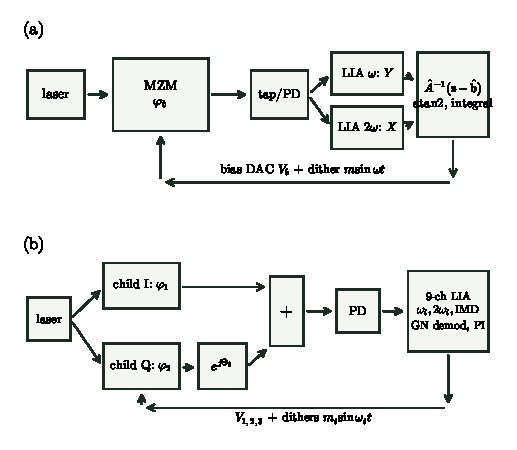
\includegraphics[width=0.62\textwidth]{figs/fig_arch.pdf}
\caption{控制架构。(a)~单~MZM：两路锁相通道馈入仿射逆与~$\atan$ 解调器。(b)~DPMZM：九路锁相通道（谐波与互调音）馈入第~\ref{sec:gn} 节的高斯--牛顿解调器。}
\label{fig:arch}
\end{figure}

\begin{figure}[!t]
\centering
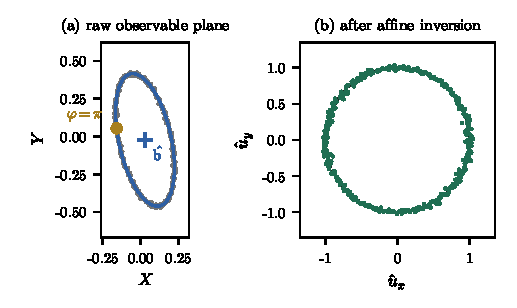
\includegraphics[width=0.62\textwidth]{figs/fig_ellipse.pdf}
\caption{标定示例：$m{=}1.2$、$\sigma{=}0.005$、$N{=}360$，含增益失配、$10^\circ$ 非正交、交叉耦合~$\varepsilon{=}0.10$ 与偏置。(a)~原始观测平面：拟合椭圆、中心~$\hat\bv$ 与~$\varphi{=}\pi$ 基准点。(b)~回拉样本~$\hat\uv=B(\zv-\hat\bv)$ 落于单位圆。}
\label{fig:ellipse}
\end{figure}

\subsection{一致增益闭环}
闭环架构如图~\ref{fig:arch}(a) 所示。取~$e=\operatorname{wrap}_{(-\pi,\pi]}(\hat\varphi_b-\varphi^\ast)$。模型成立时误差对状态\emph{恒等}线性且与目标点无关；配合常数执行斜率~$\partial\varphi_b/\partial V_b=\pi/V_\pi$，一组~PI(D) 参数对全部目标点给出相同的带宽与裕度。表~\ref{tab:schemes} 给出统一对照；传统方案静差即闭式~\eqref{eq:staticQ}--\eqref{eq:staticAM}。

\begin{table}[!t]
\caption{单~MZM 锁定方案统一对照}
\label{tab:schemes}
\centering
\footnotesize
\setlength{\tabcolsep}{5pt}
\begin{tabular}{lllll}
\toprule
方案 & 可锁点集 & 增益 & 静差 & 歧义性\\
\midrule
H2 过零（正交） & $\{\pi/2,3\pi/2\}$ & $\eta\kappa_2$ &
$(A_{12}{+}b_X)/A_{11}$ & 半周期\\
H1 过零（零/峰） & $\{0,\pi\}$ & $\eta\kappa_1$ &
$(b_Y{-}A_{21})/A_{22}$ & 半周期\\
幅值匹配 & 死区之外 & $\eta\kappa_1|\cos\varphi^\ast|$ &
式~\eqref{eq:staticAM} & $\varphi\!\leftrightarrow\!\pi{-}\varphi$\\
谐波比值 & $Y$ 非小 & 随目标点 & $\bv$ 主导 & 双象限\\
\textbf{仿射法（本文）} & $[0,2\pi)$ & 一致 & $0$（模型内） & 无\\
\bottomrule
\end{tabular}
\end{table}

\section{噪声与扰动深度设计}
\label{sec:noise}
沿切向~$\tv(\varphi)=(-\sin\varphi,\cos\varphi)^{\T}$ 对~\eqref{eq:affine} 作一阶摄动，
\begin{equation}
\sigma^2_{\hat\varphi}(\varphi)
=\tv^{\T}A^{-1}\Sigma_nA^{-\T}\tv
\xrightarrow{\Sigma_n=\sigma^2I}\sigma^2\,\tv^{\T}(A^{\T}A)^{-1}\tv
\le\frac{\sigma^2}{\sigma^2_{\min}(A)},
\label{eq:var}
\end{equation}
条件数~$\kappa(A)=\sqrt{\lambda_{\max}(M)/\lambda_{\min}(M)}$。理想链路中~$\kappa(A)=J_1(m)/J_2(m)\to 4/m$（小~$m$，图~\ref{fig:bessel}）：扰动越浅，椭圆越扁，H2 通道噪声按~$1/J_2\approx 8/m^2$ 放大；而导频自身的调制损伤~$\propto m^2$。折中由单一标量~$\kappa(A)$ 完整刻画，给出~$m$ 的设计准则。插入式估计~\eqref{eq:demod} 是一致估计但非有效估计：Fisher 信息为~$\sigma^{-2}\|A\tv\|^2$，按马氏度量向椭圆投影可达~Cram\'er--Rao 界，$\kappa(A)$ 适中时两者差异为二阶。框架并不降低特殊点\emph{处}的噪声地板——那里它复现~$\sigma_Y/(\eta\kappa_1)$ 与~$\sigma_X/(\eta\kappa_2)$——它使\emph{其余所有点}以有界噪声可达。

\begin{figure}[!t]
\centering
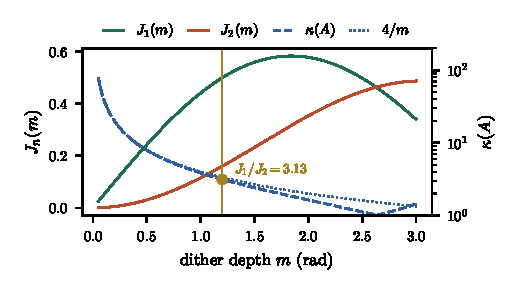
\includegraphics[width=0.58\textwidth]{figs/fig_bessel.pdf}
\caption{设计曲线：$J_1(m)$、$J_2(m)$（左轴）与条件数~$\kappa(A)$（理想链路下为~$J_1/J_2$，$m\gtrsim2.6$ 后两者互换）及其小~$m$ 渐近~$4/m$（右轴，对数）。竖线为仿真所用~$m{=}1.2$：理想比值~$J_1/J_2=3.13$；含失配的仿真真值矩阵~$\kappa(A)=2.59$。}
\label{fig:bessel}
\end{figure}

\section{推广至~DPMZM：\texorpdfstring{$\mathbb{T}^3$}{T3} 上的几何}
\label{sec:dpmzm}

\subsection{场模型与半角结构}
DPMZM 由两个子~MZM 嵌套于父干涉仪构成，偏置相位~$\phiv=(\varphi_1,\varphi_2,\varphi_3)$。无~RF 数据时
\begin{align}
E_{\mathrm{out}}&=\frac{E_{\mathrm{in}}}{2}\Bigl[\cos\frac{\Theta_1}{2}
+e^{j\Theta_3}\cos\frac{\Theta_2}{2}\Bigr],\quad \Theta_i=\varphi_i+\xi_i(t),
\nonumber\\
P_{\mathrm{out}}&=\frac{P_0}{8}\bigl[2{+}\cos\Theta_1{+}\cos\Theta_2\bigr]
+\frac{P_0}{2}\cos\frac{\Theta_1}{2}\cos\frac{\Theta_2}{2}\cos\Theta_3.
\label{eq:dpmzm}
\end{align}
括号项复现两个单~MZM 自项；干涉交叉项携带\emph{半角}因子——这是与单~MZM 的全部结构差异。三个推论立即成立：

\emph{(i)~$4\pi$ 周期。}$\cos(\varphi_1/2)$ 周期为~$4\pi$：$\varphi_1\!\to\!\varphi_1{+}2\pi$ 翻转子~I 场与交叉项符号，强度可分辨。子轴标定扫描必须跨越~$4\pi$（电压~$4V_\pi$），两倍于单~MZM 的习惯。

\emph{(ii)~Klein 等价。}子场翻号配合父相位~$\pi$ 移相只改变场的全局符号：
\begin{equation*}
T_1:(\varphi_1{+}2\pi,\ \varphi_2,\ \varphi_3{+}\pi),\qquad
T_2:(\varphi_1,\ \varphi_2{+}2\pi,\ \varphi_3{+}\pi)
\end{equation*}
二者生成~$V_4=\{\mathrm{id},T_1,T_2,T_1T_2\}$；构型空间是商~$\widetilde{\mathbb{T}}^3/V_4$（图~\ref{fig:torus}）。对~QPSK 该等价无害（星座重标记与全局相位）。

\emph{(iii)}~标准~QPSK 偏置为~$(\pi,\pi,\pm\pi/2)$（双子零点、父正交、载波抑制）；任意点运行（微波光子矢量调制、SSB 权重）把三轴停驻在一般位置。

\begin{figure}[!t]
\centering
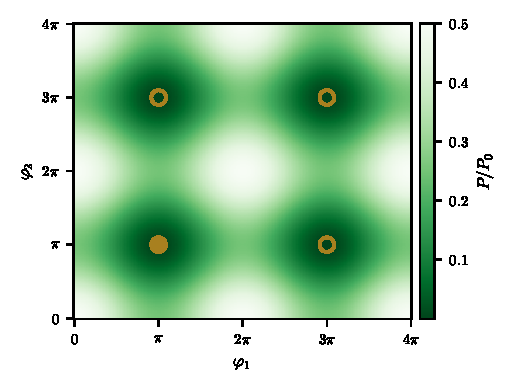
\includegraphics[width=0.55\textwidth]{figs/fig_torus.pdf}
\caption{DPMZM 强度~$P(\varphi_1,\varphi_2;\varphi_3{=}\pi/2)$，完整~$[0,4\pi)^2$ 区片。标准~QPSK 点（实心）与其三个~Klein 像（空心）强度全同——$V_4$ 商的可视化。}
\label{fig:torus}
\end{figure}

\subsection{三音谐波收获与特征映射}
施加导频~$\xi_i=m_i\sin\omega_it$ 后，自项展开系数仍为全深度~Bessel 系数~$J_n^{(i)}\triangleq J_n(m_i)$，但交叉项按\emph{半深度}系数~$j_n^{(i)}\triangleq J_n(m_i/2)$ 展开，并生成互调谱线~$\omega_1{\pm}\omega_2$、$\omega_3{\pm}\omega_1$、$\omega_3{\pm}\omega_2$——它们是携带独立信息的合法观测通道而非寄生产物。表~\ref{tab:dpchan} 列出本文采用的九通道首阶系数（$\rho P_0{=}1$、增益归一；$c_i{=}\cos\frac{\varphi_i}{2}$，$s_i{=}\sin\frac{\varphi_i}{2}$，$C_3{=}\cos\varphi_3$，$S_3{=}\sin\varphi_3$）。两点观察：交叉耦合\emph{不是}微扰（$j_1^{(1)}j_0^{(2)}J_0(m_3)\approx m_1/4$ 超过自项斜率~$J_1(m_1)/4\approx m_1/8$）；频率规划须保证集合~$\{\omega_i,2\omega_i,\omega_1{\pm}\omega_2,\omega_3{\pm}\omega_{1,2}\}$ 无碰撞（此处~$\omega_{1,2,3}=1,1.37,1.93$）。

\begin{table}[!t]
\caption{DPMZM 九通道的首阶系数}
\label{tab:dpchan}
\centering
\footnotesize
\setlength{\tabcolsep}{5pt}
\begin{tabular}{llll}
\toprule
通道 & 频率 & 首阶系数~$\times$ 单项式 & 角色\\
\midrule
$Y_1$ & $\omega_1$ & $-\frac14J_1^{(1)}\sin\varphi_1-j_1^{(1)}j_0^{(2)}J_0(m_3)\,s_1c_2C_3$ & 子~I 锁定\\
$X_1$ & $2\omega_1$ & $+\frac14J_2^{(1)}\cos\varphi_1+j_2^{(1)}j_0^{(2)}J_0(m_3)\,c_1c_2C_3$ & 判别\\
$Y_2$ & $\omega_2$ & $-\frac14J_1^{(2)}\sin\varphi_2-j_0^{(1)}j_1^{(2)}J_0(m_3)\,c_1s_2C_3$ & 子~Q 锁定\\
$X_2$ & $2\omega_2$ & $+\frac14J_2^{(2)}\cos\varphi_2+j_0^{(1)}j_2^{(2)}J_0(m_3)\,c_1c_2C_3$ & 判别\\
$Y_3$ & $\omega_3$ & $-j_0^{(1)}j_0^{(2)}J_1(m_3)\,c_1c_2S_3$ & 父（注意~$c_1c_2$）\\
$X_3$ & $2\omega_3$ & $+j_0^{(1)}j_0^{(2)}J_2(m_3)\,c_1c_2C_3$ & 父判别\\
$Z_-$ & $\omega_1{-}\omega_2$ & $+j_1^{(1)}j_1^{(2)}J_0(m_3)\,s_1s_2C_3$ & Kawakami 型~\cite{kawakami2012}\\
$Z_{13}$ & $\omega_3{-}\omega_1$ & $+j_1^{(1)}j_0^{(2)}J_1(m_3)\,s_1c_2S_3$ & 本文引入\\
$Z_{23}$ & $\omega_3{-}\omega_2$ & $+j_0^{(1)}j_1^{(2)}J_1(m_3)\,c_1s_2S_3$ & 本文引入\\
\bottomrule
\end{tabular}
\end{table}

对三个相位各应用一次引理~\ref{lem:fact}（半角版本逐字成立），并三线性展开交叉项，光电流的~$\phiv$ 依赖只能由十二个三角单项式构成：
\begin{align}
\Phi(\phiv)&=\bigl(\underbrace{\cos\varphi_1,\sin\varphi_1,
\cos\varphi_2,\sin\varphi_2}_{\text{自项（全角）}},\;
\underbrace{\vv_1{\otimes}\vv_2{\otimes}\vv_3}_{\text{交叉项，8 维}}
\bigr),\nonumber\\
\vv_1&=(c_1,s_1),\quad \vv_2=(c_2,s_2),\quad \vv_3=(C_3,S_3).
\label{eq:feature}
\end{align}

\begin{theorem}[DPMZM 精确仿射性]
\label{th:dpmzm}
对任意周期导频波形组~$\{\xi_i\}$、任意线性接收链与任意一组~$K$ 个线性解调泛函，
\begin{equation}
\zv=A\,\Phi(\phiv)+\bv+\nv,\qquad A\in\mathbb{R}^{K\times 12}
\label{eq:dpaffine}
\end{equation}
精确成立。理想链路下~$A=A_0$ 由表~\ref{tab:dpchan} 给出，且高度稀疏（每行一至二个非零元，图~\ref{fig:ahat}）。
\end{theorem}

定理伴随一个方法论转变：一维情形我们逐项枚举非理想机理；三维情形黑箱仿射辨识吸收\emph{全部}线性失配，机理枚举让位于结构定理。规范群同样逐字推广：相位平移~$\varphi_i\to\varphi_i+\alpha_i$ 经三角加法公式在特征空间上诱导\emph{线性}作用（半角对按~$\alpha_i/2$ 旋转、全角对按~$\alpha_i$ 旋转、张量块按张量旋转），故~$(A,\bv)$ 只能辨识到三个相位原点——逐轴由直流回归固定，与第~\ref{sec:calib} 节完全相同——外加反射（扫描定向）与离散~$V_4$（基本域约定）。表~\ref{tab:struct} 总结对应关系。

\begin{table}[!t]
\caption{结构对应：单~MZM 与~DPMZM}
\label{tab:struct}
\centering
\footnotesize
\setlength{\tabcolsep}{3pt}
\begin{tabular}{lll}
\toprule
要素 & 单~MZM & DPMZM\\
\midrule
状态流形 & $\mathbb{S}^1$ & $\mathbb{T}^3$（构型~$\widetilde{\mathbb{T}}^3/V_4$）\\
特征映射 & $\uv\in\mathbb{R}^2$（恒等） & $\Phi\in\mathbb{R}^{12}$（含半角）\\
轴向周期 & $2\pi$ & 子轴~$4\pi$，父轴~$2\pi$\\
通道数 & 2（$\omega,2\omega$） & $\ge 7$，IMD 必需\\
曲面拟合 & 椭圆（二次簇） & 准周期扫描回归\\
规范群 & $O(2)$ & $\mathbb{T}^3\rtimes(\text{反射}\times V_4)$\\
解调 & $\atan$（闭式） & 热启动高斯--牛顿\\
失明修复 & H1/H2 联用 & IMD 通道\\
\bottomrule
\end{tabular}
\end{table}

\section{可观测性与~IMD 通道的必然性}
\label{sec:obs}
解调的局部可行性由观测雅可比~$\Jc(\phiv)=A\,D\Phi(\phiv)\in\mathbb{R}^{K\times3}$ 的秩条件~$\sigma_{\min}(\Jc)>0$ 刻画——命题~\ref{prop:rolle} 浸入论证的直接推广。与圆不同，$\mathbb{T}^3$ 的\emph{被观测}嵌入可以退化，而且恰好在最糟的地方退化。

\begin{proposition}[标准点失明及其奇异轨迹]
\label{prop:blind}
取表~\ref{tab:dpchan} 中六个谐波通道~$Y_{1,2,3},X_{1,2,3}$ 与理想~$A_0$。使~$\partial\zv/\partial\varphi_3=\mathbf{0}$（父轴不可观）的集合恰为~$\{c_1=c_2=0\}$，即\emph{标准~QPSK 工作点的~Klein 轨道}，且对一切~$\varphi_3$ 成立。加入~IMD 通道~$Z_-$（单项式~$s_1s_2C_3$，其~$\varphi_3$ 偏导在标准点为~$-s_1s_2S_3=\mp1$）即在该处恢复满秩。
\end{proposition}
\begin{proof}[证明梗概]
六通道所含交叉单项式的~$\varphi_3$ 偏导（略去正的深度系数）分别为~$-s_1c_2S_3$（$Y_1$）、$-c_1s_2S_3$（$Y_2$）、$-c_1c_2S_3$（$X_1,X_2,X_3$）与~$+c_1c_2C_3$（$Y_3$）。对一切~$\varphi_3$ 同时为零要求~$s_1c_2=c_1s_2=c_1c_2=0$，唯一解为~$c_1=c_2=0$（另一支~$s_1=s_2=0$ 与~$c_1c_2=0$ 矛盾）。数值上，标准点处六通道~$\sigma_{\min}=1.3\times10^{-9}$（机器零），加入~$Z_-$ 后~$5.5\times10^{-2}$。
\end{proof}

传统通道集因此不是“偶尔”退化：它\emph{恰好}在每台~QPSK 发射机的标准工作点失明。文献中以~IMD 检测父偏置的做法~\cite{kawakami2012} 由此成为秩条件的必然要求。为完整起见，须指出一处残余奇点：在~$\{c_1{=}c_2{=}0,\ S_3{=}0\}$（如~$(\pi,\pi,0)$，输出全暗）处，全部~$\varphi_3$ 偏导落在唯一未被观测的单项式~$s_1s_2S_3$ 上，九通道下~$\sigma_{\min}=1.1\times10^{-17}$；三阶~IMD~$\omega_1{+}\omega_2{\pm}\omega_3$ 或路径绕行可消解。图~\ref{fig:obs} 给出~$[0,4\pi)^2$ 上的~$\log_{10}\sigma_{\min}(\Jc)$：六通道的暗斑落在~Klein 轨道上，九通道在~$\varphi_3=\pi/2$ 处完全修复，而~$\varphi_3=0$ 切片上预言的残余奇点重现。

\begin{figure}[!t]
\centering
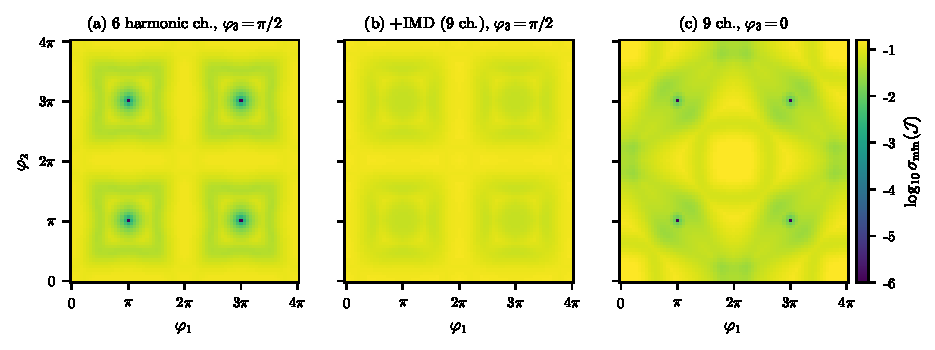
\includegraphics[width=0.92\textwidth]{figs/fig_obs.pdf}
\caption{可观测性热图~$\log_{10}\sigma_{\min}(\Jc)$，$(\varphi_1,\varphi_2)\in[0,4\pi)^2$。(a)~六谐波通道、$\varphi_3{=}\pi/2$：暗斑恰落在标准~QPSK 点的~Klein 轨道上。(b)~加入三个~IMD 通道后修复。(c)~九通道、$\varphi_3{=}0$：命题~\ref{prop:blind} 的残余奇点在同一轨道上重现。}
\label{fig:obs}
\end{figure}

\section{\texorpdfstring{$\mathbb{T}^3$}{T3} 上的标定与高斯--牛顿解调}
\label{sec:gn}
单~MZM 的标定利用了“模型曲面是二次簇”这一巧合。$\Phi(\mathbb{T}^3)$ 不再是二次簇，几何拟合失去闭式——但定理给出补偿：观测对特征\emph{线性}，故在规范固定坐标下辨识就是普通最小二乘
\begin{equation}
[\hat A\,|\,\hat\bv]
=\Bigl(\sum_k\zv_k\tilde\Phi_k^{\T}\Bigr)
\Bigl(\sum_k\tilde\Phi_k\tilde\Phi_k^{\T}\Bigr)^{-1},\quad
\tilde\Phi=\begin{pmatrix}\Phi\\1\end{pmatrix},
\label{eq:regress}
\end{equation}
一次~$13{\times}13$ Gram 分解服务全部~$K$ 个通道。三维网格扫描不必要：取增量比无理的\emph{准周期}轨线~$\varphi_i(k)=k\Delta_i$（此处~$\Delta=(0.0424,0.0532,0.0679)$），单条轨线遍历性地填充~$\mathbb{T}^3$，$N=3000$ 个样本即得良态~Gram 矩阵。各轴标度~$V_{\pi,i}$ 由扫描数据的基波周期估计获得（子轴周期~$4\pi$），绝对原点——$\mathbb{T}^3$ 规范——由逐轴直流回归固定，与前同。

解调则推广~$\atan$（图~\ref{fig:arch}(b)）：后者存在是因为圆嵌入有全局闭式逆，$\Phi(\mathbb{T}^3)$ 没有；但控制是\emph{跟踪}问题，上一周期估计热启动阻尼高斯--牛顿步~\cite{nocedal2006}
\begin{equation}
\hat\phiv\leftarrow\hat\phiv+(\Jc^{\T}\Jc+\lambda I)^{-1}
\Jc^{\T}\bigl[\zv-\hat A\Phi(\hat\phiv)-\hat\bv\bigr],
\label{eq:gn}
\end{equation}
两次迭代即达测量噪声地板；收敛域由~$\sigma_{\min}(\Jc)$ 与嵌入曲率界共同给出，故图~\ref{fig:obs} 同时是收敛域地图。借助~$\hat A$ 的稀疏性，每控制周期约数百次乘加加一次~$3{\times}3$ 求解——相对锁相处理本身在~Cortex-M 级控制器上可忽略。误差~$\mathbf{e}=\hat\phiv-\phiv^\ast$ 再次严格线性、三轴解耦、目标无关。

\emph{噪声地板与扰动深度设计。}估计协方差为~Cram\'er--Rao 型~$\Sigma_{\hat\phiv}=(\Jc^{\T}\Sigma_n^{-1}\Jc)^{-1}$，其~$K{=}2$ 时的插入式对应即式~\eqref{eq:var}。与单~MZM 不同，条件数此时由二阶小的~IMD 系数主导：双子零点附近父相位方差
\begin{equation}
\sigma^2_{\hat\varphi_3}\approx
\frac{\sigma^2}{\bigl[j_1^{(1)}j_1^{(2)}J_0(m_3)\bigr]^2}
\approx\Bigl(\frac{16}{m_1m_2}\Bigr)^{2}\sigma^2,
\label{eq:parentnoise}
\end{equation}
比子轴地板~$(8/m)^2\sigma^2$ 高一个量级以上，且对~$1/m$ 的依赖由一次方升为二次方。扰动深度因此由父轴~IMD 信噪比而非子轴决定，最优取值显著高于单~MZM 的习惯。

对照基线取文献式三独立环：误差量~$(Y_1,Y_2,Z_-)$、参考值由理想模型~$A_0\Phi(\phiv^\ast)$ 计算、斜率取理想雅可比的\emph{对角元}——即承认理想耦合但放弃矩阵求逆，且对~$A\neq A_0$、$\bv\neq0$ 无知。在标准点附近它不受耦合之苦（交叉项在该点局部消失，教科书设计的成立条件由此获得几何解释），但第~\ref{sec:conventional} 节的静差原样继承，且被二阶小的父轴斜率~$j_1^{(1)}j_1^{(2)}J_0(m_3)$ 放大；在任意目标点处，再叠加跨轴耦合与死区。

\begin{figure}[!t]
\centering
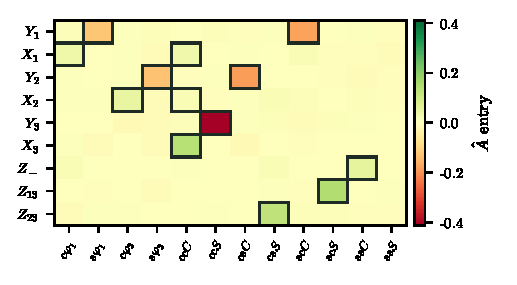
\includegraphics[width=0.6\textwidth]{figs/fig_ahat.pdf}
\caption{DPMZM 黑箱辨识：回归所得~$\hat A$（色块）对照理想~$A_0$ 的稀疏指纹（方框）。指纹外的元素是注入的非结构化扰动~$\delta_A{=}0.12$，被回归如实捕获。}
\label{fig:ahat}
\end{figure}


\section{基于仿射模型的偏压控制算法设计}
\label{sec:algo}
前述理论落地为一个由监督状态机组织的两阶段算法（图~\ref{fig:flow}）：\emph{标定阶段}执行扫描、拟合与规范固定并完成自检；\emph{运行阶段}每控制周期执行解调--误差--PI 更新，同时以模型残差作为失配监视量，越限即触发重定标，构成闭合的自维护回路。两阶段分别由算法~\ref{alg:cal} 与算法~\ref{alg:run} 给出；单~MZM 与~DPMZM 共享同一骨架，仅在拟合方式（椭圆几何拟合对线性回归）与解调算子（$\atan$ 对两步高斯--牛顿）处分支。

\begin{figure}[!t]
\centering
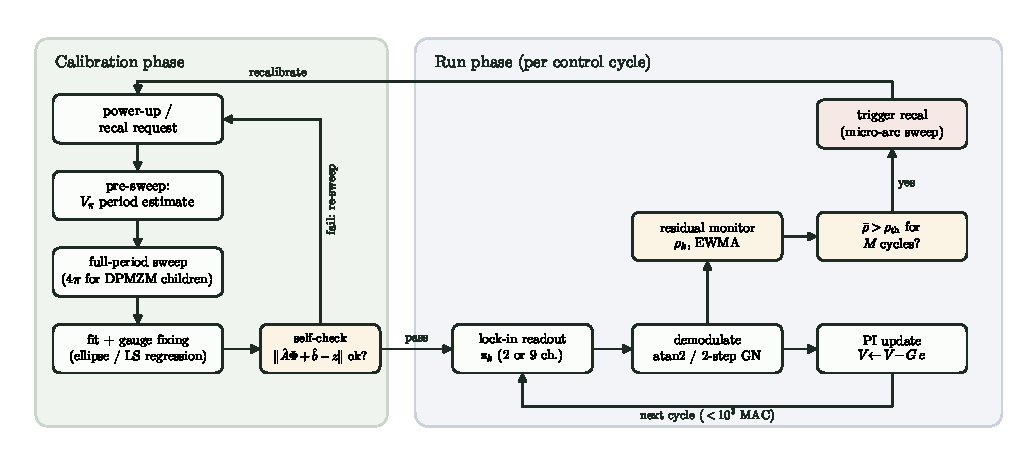
\includegraphics[width=0.95\textwidth]{figs/fig_flow.pdf}
\caption{监督状态机：左为标定阶段（扫描$\to$拟合与规范固定$\to$自检），右为运行阶段的每周期回路（锁相读出$\to$解调$\to$PI$\to$残差监测），残差越限持续~$M$ 周期即触发微幅弧重定标并返回标定通道。}
\label{fig:flow}
\end{figure}

\begin{algorithm}[!t]
\caption{自标定与规范固定（上电或重定标触发时执行）}
\label{alg:cal}
\begin{algorithmic}[1]
\Require 样本数~$N$；通道集（MZM：$K{=}2$；DPMZM：$K{=}9$，含~IMD）
\Ensure 解调参数（MZM：$B,\hat\bv$；DPMZM：$\hat A,\hat\bv$）与残差阈值~$\rho_{\rm th}$
\State 预扫描估计各轴~$V_{\pi,i}$（基波周期；DPMZM 子轴按~$4\pi$ 周期）
\State 满周期扫描记录~$\{\zv_k,\bar\imath_k\}_{k=1}^N$（DPMZM 取准周期轨线~$\varphi_i(k)=k\Delta_i$，增量比无理）
\If{单~MZM}
  \State 中心化/归一后代数最小二乘拟合锥曲线~$\Rightarrow$ 中心~$\hat\bv$ 与~$M\succ0$；$B_0\gets M^{1/2}$
  \State 由轨道环绕方向定反射~$F$；直流序列对~$(1,\cos\theta_k,\sin\theta_k)$ 回归得~$\hat\varphi_c$；$B\gets R(-\hat\varphi_c)FB_0$
\Else\Comment{DPMZM}
  \State 构造~$\tilde\Phi_k=(\Phi(\phiv_k)^{\T},1)^{\T}$；解~$13{\times}13$ 法方程得~$[\hat A\,|\,\hat\bv]$（式~\eqref{eq:regress}）
  \State 逐轴直流回归固定三个相位原点；按基本域约定消解~$V_4$ 歧义
\EndIf
\State 自检：$\max_k\|\zv_k-\hat A\Phi_k-\hat\bv\|<\epsilon_{\rm cal}$？不通过则重新扫描
\State 记录残差统计~$(\mu_\rho,\sigma_\rho)$，置~$\rho_{\rm th}=\mu_\rho+k_\sigma\sigma_\rho$（$k_\sigma\approx4$--$6$）
\end{algorithmic}
\end{algorithm}

\begin{algorithm}[!t]
\caption{运行时控制周期（含残差监测与重定标触发）}
\label{alg:run}
\begin{algorithmic}[1]
\Require 目标~$\phiv^\ast$、环路增益~$G$、阈值对~$(\rho_{\rm th},M)$、上周期估计~$\hat\phiv^-$
\State 读取锁相输出~$\zv_k$
\If{单~MZM}
  \State $\hat\uv\gets B(\zv_k-\hat\bv)$；\quad $\hat\varphi\gets\atan(\hat u_y,\hat u_x)$；\quad $\rho_k\gets\bigl|\,\|\hat\uv\|-1\bigr|$
\Else\Comment{DPMZM}
  \State 以~$\hat\phiv^-$ 热启动执行两步阻尼高斯--牛顿（式~\eqref{eq:gn}）得~$\hat\phiv$；$\rho_k\gets\|\zv_k-\hat A\Phi(\hat\phiv)-\hat\bv\|$
\EndIf
\State $\mathbf e\gets\operatorname{wrap}(\hat\phiv-\phiv^\ast)$；\quad PI 更新~$V\gets V-G\,\mathbf e\cdot V_\pi/\pi$ 写入偏压~DAC
\State 残差~EWMA：$\bar\rho\gets(1-\lambda)\bar\rho+\lambda\rho_k$
\If{$\bar\rho>\rho_{\rm th}$ 连续~$M$ 周期}
  \State 保持当前~$V$，执行微幅弧重定标（调用算法~\ref{alg:cal}；DPMZM 弧优先激励~$s_1s_2$ 子空间）
\EndIf
\Ensure 进入下一周期；全周期代价~$<10^3$ 次乘加
\end{algorithmic}
\end{algorithm}

三处整定与实现要点。\emph{阈值整定}：$\rho_{\rm th}$ 直接取自标定末尾的残差分布而非人为设定，配合~EWMA（$\lambda\approx0.05$）与连续~$M$ 周期判决（$M\approx20$--$30$），误触发率由高斯尾界控制在可忽略水平，检测延迟约~$M+1/\lambda$ 个周期量级。\emph{重定标弧}：幅度~$\pm0.3$~rad 量级的微幅弧足以重新张成局部可辨识子空间；期间偏压保持上一值，对承载业务的扰动等同于一次常规导频包络。\emph{定点化}：$\atan$ 以~CORDIC 或查表实现；高斯--牛顿的~$3{\times}3$ 求解用~Cholesky 展开为定值乘加序列；全部参数存储为~MZM 六个标量、DPMZM 共~$9{\times}12{+}9{=}117$ 个标量，置于配置页即可。

\section{数值验证}
\label{sec:numerics}

\subsection{仿真设置与主要结果}
所有仿真由扰动真值~$A_{\mathrm{true}}=A_0+\delta_A\,\Delta A$、$\bv_{\mathrm{true}}=\delta_b\,\Delta\bv$ 生成数据（固定伪随机~$\Delta A,\Delta\bv$；$\delta_A{=}0.12$ 为相对~Frobenius 尺度，$\delta_b$ 对应~${\sim}10^{-2}$ 量级偏置），叠加逐通道高斯噪声与共同漂移序列（随机游走加慢正弦），对受比较的控制器施加同源漂移。单~MZM 参数：$m{=}1.2$、$g_X{=}1.18$、$g_Y{=}0.88$、$\delta{=}10^\circ$、$\varepsilon{=}0.10$、$\bv=(0.030,-0.022)$、$\sigma{=}0.005$、$N{=}360$；DPMZM：$m_i{=}1.2$、$\sigma{=}0.002$、$N{=}3000$。结果汇总于表~\ref{tab:results}。

\begin{table}[!t]
\caption{数值验证汇总}
\label{tab:results}
\centering
\footnotesize
\setlength{\tabcolsep}{5pt}
\begin{tabular}{ll}
\toprule
量 & 结果\\
\midrule
\multicolumn{2}{l}{\emph{单~MZM}}\\
零噪声解调误差（全周期） & $0.0000$~mrad（机器精度）\\
零噪声~$\hat A$ 对真值~$A$ & Frobenius 误差~$0.00\%$\\
含噪标定解调偏差（$\sigma{=}0.005$） & 中位~$2.35$、P95~$6.25$~mrad\\
规范固定：直流回归对~argmin & ${\sim}2$ 对~${\sim}42$~mrad\\
闭环（$\varphi^\ast{=}1.9$） & 仿射~$12.7$ / H1 匹配~$1315$~mrad（rms）\\
$m{=}1.2$ 处的~$\kappa(A)$（受扰真值） & $2.59$（理想比值~$3.13$）\\
\midrule
\multicolumn{2}{l}{\emph{DPMZM}}\\
$D\Phi$ 对有限差分 & 最大~$8\times10^{-10}$\\
Klein 不变性~$\|\Phi\circ T_1-\Phi\|$ & $2\times10^{-15}$\\
零噪声辨识 / GN 恢复 & $2.4\times10^{-13}\%$ / $6\times10^{-12}$~mrad\\
含噪辨识（$\sigma{=}0.002$）/ 解调偏差 & $0.17\%$ / 中位~$1.9$、P95~$3.8$~mrad\\
$\sigma_{\min}$：六通道 / 九通道（标准点） & $1.3\times10^{-9}$ / $5.5\times10^{-2}$\\
$\sigma_{\min}$：九通道于~$(\pi,\pi,0)$ & $1.1\times10^{-17}$\\
闭环（任意目标点） & GN~$17.2$ / 三环~$358$~mrad（rms）\\
闭环（标准目标点） & GN~$18.5$ / 三环~$397$~mrad（rms）\\
三环静差，30 个失配实现 & 标准点：中位~$292$~[184,393]~mrad\\
 & 任意点：$23/30$ 失锁；余者中位~$417$~mrad\\
\midrule
\multicolumn{2}{l}{\emph{算法级动态（第~\ref{sec:algo} 节算法）}}\\
捕获时间常数（理论~$1/G$） & 四目标重合于~$(1-G)^n$，$5.6$ 周期\\
阶跃整定（至~$20$~mrad） & $20$--$22$ 周期，与目标点无关\\
漂移突变：检测延迟 / 恢复 & $31$ 周期 / $13.7$~mrad（突变前~$12.6$）\\
\bottomrule
\end{tabular}
\end{table}

四个结果值得强调。其一，零噪声闭合（辨识~$10^{-13}\%$、由~$0.3$~rad 热启动偏差恢复至~$10^{-12}$~mrad）证实定理~\ref{th:affine} 与定理~\ref{th:dpmzm} 是精确命题而非近似。其二，闭环对比（图~\ref{fig:mzmloop} 与图~\ref{fig:dploop}）呈现理论预言的分层失效：单~MZM 任意目标点处~H1 方案锁入错误分支，图~\ref{fig:sweep} 进一步将该单点对比扩展到整个目标相位网格——传统方案的闭式静差在各自死区附近发散，仿射环路的实测~rms 在全部目标上平坦，其逐相位噪声地板与式~\eqref{eq:var} 吻合；DPMZM 三环基线在两类目标点均收敛，但携带数百毫弧度静差——未被辨识的~$(\Delta A,\bv)$ 经二阶小的父轴斜率转化而来；对~30 个失配实现的蒙特卡洛（图~\ref{fig:mcdp}）给出标准点中位静差~$292$~mrad（IQR~$184$--$393$）；任意点处~$23/30$ 个实现完全失锁，未失锁者中位静差仍达~$417$~mrad——而高斯--牛顿仿射控制器在所有情形保持~$16$--$19$~mrad（rms），仅受测量噪声限制。其三，可观测性热图（图~\ref{fig:obs}）精确可视化命题~\ref{prop:blind}：六通道盲斑落在标准点的~Klein 轨道上，被~IMD 通道修复，预言的残余奇点在~$S_3{=}0$ 切片上重现。其四，规范固定对照（图~\ref{fig:gauge}）从数值上证实第~\ref{sec:calib} 节的论断：直流回归规范的标定偏差中位约~$2$~mrad 并按~$N^{-1/2}$ 收缩，而~argmin 基准受平坦极小值限制停滞在数十~mrad。

\begin{figure}[!t]
\centering
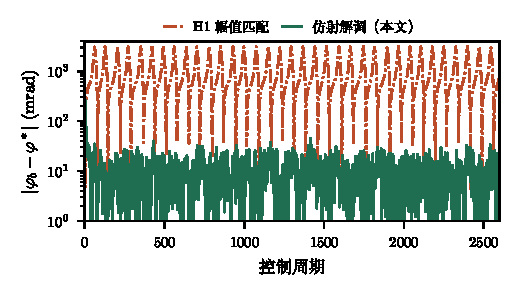
\includegraphics[width=0.58\textwidth]{figs/fig_mzmloop.pdf}
\caption{单~MZM 闭环：任意目标点~$\varphi^\ast{=}1.9$~rad，同源漂移，$\sigma{=}0.005$（对数误差轴）。仿射解调保持~$12.7$~mrad 均方根；H1 幅值匹配锁入错误分支，误差徘徊于数百毫弧度至弧度级（静差~${\sim}1.3$~rad）。}
\label{fig:mzmloop}
\end{figure}

\begin{figure}[!t]
\centering
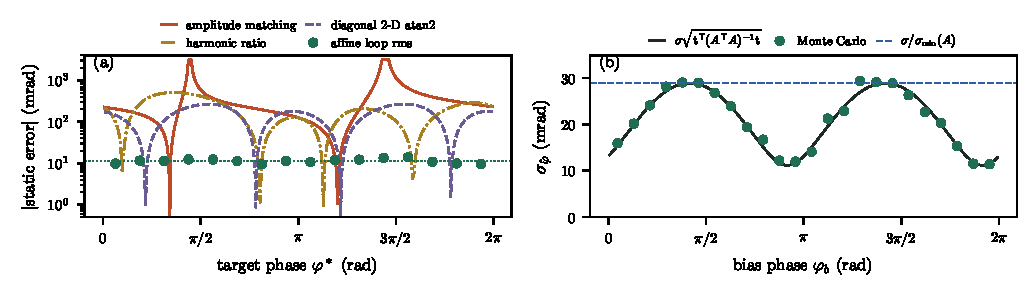
\includegraphics[width=0.92\textwidth]{figs/fig_sweep.pdf}
\caption{任意点性能随目标相位的分布。(a)~传统两类方案的闭式静差（幅值匹配为式~\eqref{eq:staticAM}，谐波比值为锁定条件的数值根）在各自死区附近发散，仿射环路的实测闭环~rms（圆点，含同源漂移与噪声）在全部目标上平坦；(b)~解调噪声地板随相位的分布：式~\eqref{eq:var} 理论曲线、蒙特卡洛实测与上界~$\sigma/\sigma_{\min}(A)$。}
\label{fig:sweep}
\end{figure}

\begin{figure}[!t]
\centering
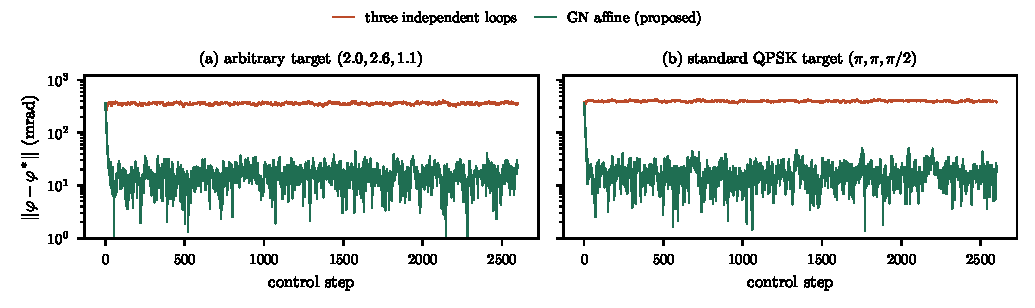
\includegraphics[width=0.85\textwidth]{figs/fig_dploop.pdf}
\caption{DPMZM 闭环跟踪，同源漂移，$\sigma{=}0.002$、$\delta_A{=}0.12$（对数误差轴）。(a)~任意目标点：三环基线携带~${\sim}0.36$~rad 静差；(b)~即使在标准~QPSK 点，基线仍经二阶小的父轴斜率继承可比静差，而高斯--牛顿仿射控制器在两处均保持~${\sim}18$~mrad（rms）。}
\label{fig:dploop}
\end{figure}

\begin{figure}[!t]
\centering
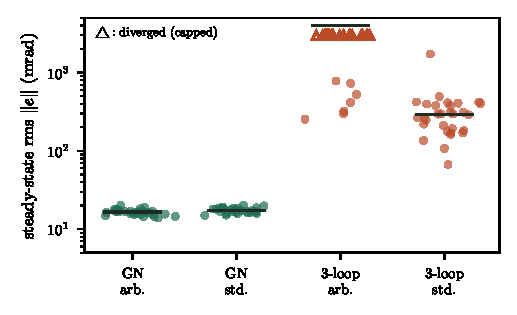
\includegraphics[width=0.58\textwidth]{figs/fig_mcdp.pdf}
\caption{DPMZM 静差的蒙特卡洛分布（30 个失配实现，横杠为中位数）：高斯--牛顿仿射控制器在任意与标准目标处均停留在测量噪声地板；三环基线携带数百毫弧度静差，且在任意目标处出现发散实现（三角标记，截幅显示）。}
\label{fig:mcdp}
\end{figure}

\begin{figure}[!t]
\centering
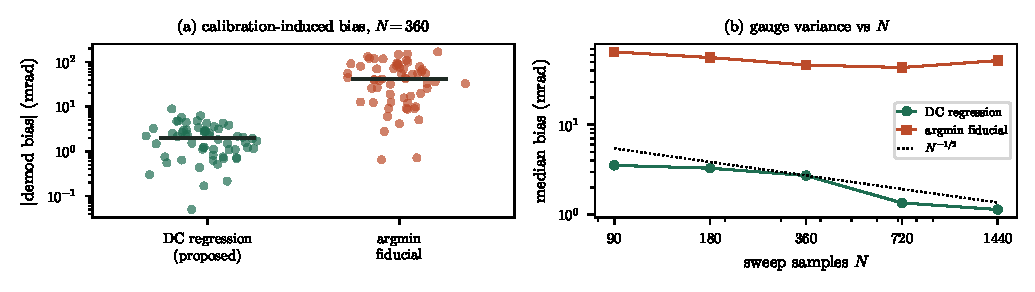
\includegraphics[width=0.92\textwidth]{figs/fig_gauge.pdf}
\caption{规范固定方案对照。(a)~$N{=}360$ 时标定引入的解调偏差分布：直流回归规范对~argmin 基准（横杠为中位数）；(b)~偏差中位数随扫描样本数~$N$ 的标度：回归规范按~$N^{-1/2}$ 收缩，argmin 基准受平坦极小值限制几乎不收缩。}
\label{fig:gauge}
\end{figure}


\subsection{算法级行为验证}
图~\ref{fig:acq}--\ref{fig:recal} 验证算法~\ref{alg:cal}--\ref{alg:run} 的三项动态性质。\emph{捕获瞬态}（图~\ref{fig:acq}）：从~$1.5$~rad（MZM）与~$\|\Delta\phiv\|\approx0.96$~rad（DPMZM）的初始偏差出发，四个相距甚远的~MZM 目标点的误差衰减曲线彼此重合，并与理论包络~$(1-G)^n$ 一致——时间常数~$1/G\approx5.6$ 个周期、与目标点无关，这是“一致增益”结论的最直接动态验证；DPMZM 在任意点与标准点同样重合于~$(1-G)^n$。\emph{设定点阶跃序列}（图~\ref{fig:step}）：MZM 目标在五个任意相位间阶跃，各步进入~$20$~mrad 误差带的整定时间为~$20$--$22$ 个周期，逐步一致；DPMZM 三轴联合阶跃表现相同。\emph{残差触发重定标}（图~\ref{fig:recal}）：在第~$1200$ 周期注入漂移突变（$g_X{:}\,1.18\!\to\!0.85$ 且~$b_x$ 跳变，模拟功率/扰动深度突变），圆残差~EWMA 越过阈值~$\rho_{\rm th}{=}0.06$，经~$31$ 个周期判决延迟触发重定标；失配期锁定误差升至~$275$~mrad（rms），重定标后恢复至~$13.7$~mrad，与突变前的~$12.6$~mrad 一致——自维护回路闭合。

\begin{figure}[!t]
\centering
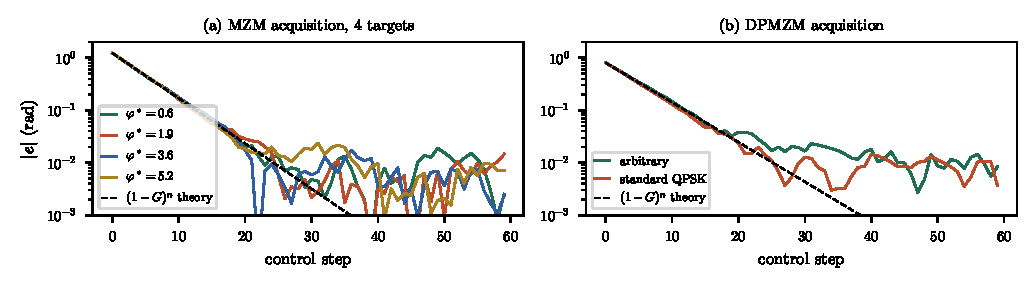
\includegraphics[width=0.92\textwidth]{figs/fig_acq.pdf}
\caption{捕获瞬态与一致增益验证。(a)~单~MZM：四个任意目标点（自~$1.5$~rad 偏差捕获）的误差曲线相互重合并贴合理论包络~$(1-G)^n$；(b)~DPMZM：任意目标与标准~QPSK 目标同样重合。}
\label{fig:acq}
\end{figure}

\begin{figure}[!t]
\centering
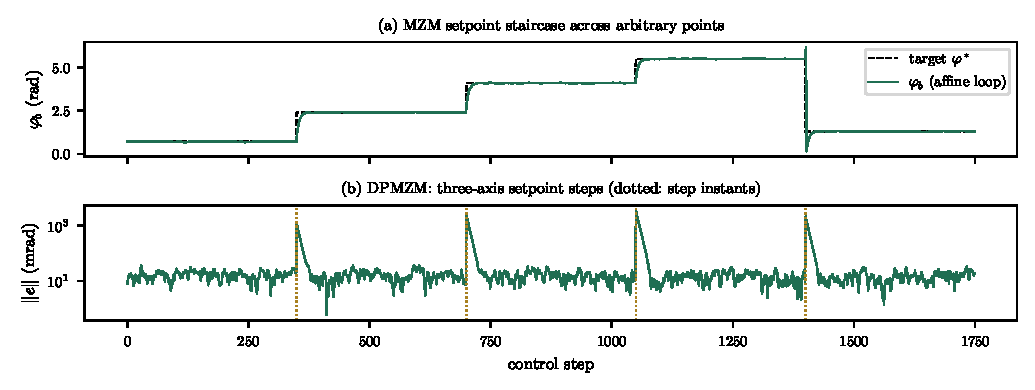
\includegraphics[width=0.92\textwidth]{figs/fig_step.pdf}
\caption{设定点阶跃序列。(a)~MZM：目标在五个任意相位间阶跃，各步整定~$20$--$22$ 周期（至~$20$~mrad）且逐步一致；(b)~DPMZM 三轴联合阶跃的误差范数（虚线为阶跃时刻）。}
\label{fig:step}
\end{figure}

\begin{figure}[!t]
\centering
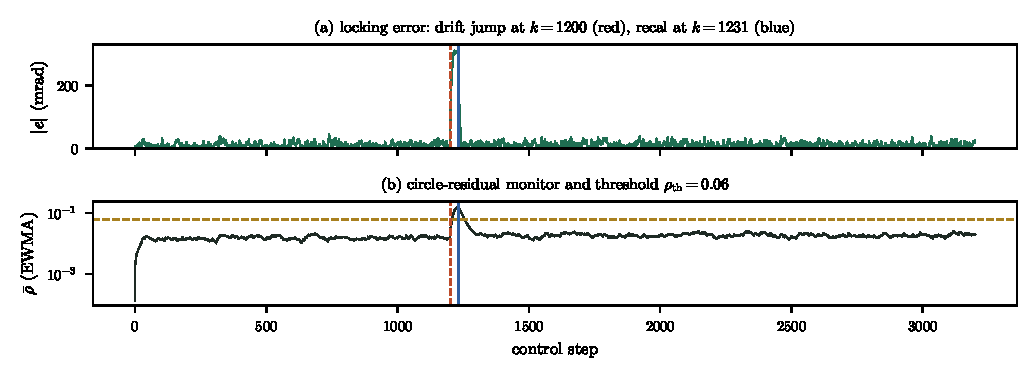
\includegraphics[width=0.85\textwidth]{figs/fig_recal.pdf}
\caption{残差触发重定标。第~$1200$ 周期注入漂移突变（红虚线），(b)~中圆残差~EWMA 越过阈值~$\rho_{\rm th}{=}0.06$（金虚线），延迟~$31$ 周期后触发重定标（蓝线）；(a)~中锁定误差由失配期的~$275$~mrad 恢复至~$13.7$~mrad。}
\label{fig:recal}
\end{figure}

\section{实验验证（占位）}
\label{sec:exp}
本节为预留结构：实验平台与测试矩阵已确定，数据待测试完成后填入；占位图框（图~\ref{fig:exp1}--图~\ref{fig:exp3}）标注了每张图对应的测量内容与其仿真对照。

\emph{平台规划。}实验在既有~STM32G474 双谐波（H1/H2）软件锁相偏压控制固件基础上以纯软件方式升级：偏压由~AD5676R 16~bit DAC 产生，监测链为~InGaAs PD 加跨阻放大，被测器件为~LiNbO$_3$ 单驱~MZM（第一阶段）与~DPMZM（第二阶段，新增~IMD 通道锁相与~$9{\times}12$ 稀疏高斯--牛顿步）；导频频率取~kHz 量级，控制周期~$1$--$10$~ms，标定参数存储于配置页。测试矩阵见表~\ref{tab:exp}。

\begin{table}[!t]
\caption{实验测试矩阵（仿真对照值来自表~\ref{tab:results}；实验列待测）}
\label{tab:exp}
\centering
\footnotesize
\setlength{\tabcolsep}{6pt}
\begin{tabular}{lll}
\toprule
指标 & 仿真值 & 实验值\\
\midrule
标定后无噪自检残差（MZM） & 中位~$2.35$~mrad & 待测\\
任意点锁定精度~rms（$\varphi^\ast$ 网格扫描） & $12.7$~mrad@$1.9$~rad & 待测\\
捕获整定时间（至~$20$~mrad） & $20$--$22$ 周期 & 待测\\
漂移突变检测延迟 / 恢复 & $31$ 周期 / $13.7$~mrad & 待测\\
$24$~h 长期稳定性（含重定标事件数） & --- & 待测\\
DPMZM 任意点三轴~rms & $17.2$~mrad & 待测\\
\bottomrule
\end{tabular}
\end{table}

\begin{figure}[!t]
\centering
\placeholderbox{3.6cm}{实测标定数据：观测平面椭圆、拟合曲线与回拉单位圆\\（与仿真图~\ref{fig:ellipse} 对照；标注~$\hat A$、$\hat\bv$、$\kappa(\hat A)$ 实测值）}
\caption{【占位】单~MZM 实测标定结果。}
\label{fig:exp1}
\end{figure}

\begin{figure}[!t]
\centering
\placeholderbox{3.6cm}{任意点锁定精度扫描：$\varphi^\ast$ 取~$[0,2\pi)$ 网格（$\ge16$ 点），\\每点锁定~rms 与静差对比~H1 幅值匹配基线（与图~\ref{fig:mzmloop} 对照）}
\caption{【占位】任意点锁定精度随目标相位的分布。}
\label{fig:exp2}
\end{figure}

\begin{figure}[!t]
\centering
\placeholderbox{3.6cm}{$24$~h 长期运行记录：锁定误差、残差监视量~$\bar\rho$、\\重定标触发事件与环境温度同步曲线（与图~\ref{fig:recal} 对照）}
\caption{【占位】长期稳定性与自维护回路实测。}
\label{fig:exp3}
\end{figure}

\section{讨论}
\label{sec:discussion}
\emph{持续激励。}闭环稳态下~$\phiv$ 停驻一点，$(A,\bv)$ 失去可观性——基于辨识的方案共有的问题~\cite{ljung1999}。实用对策：残差监测~$\|\zv-\hat A\Phi(\hat\phiv)-\hat\bv\|$ 作为失配告警触发重定标；周期性微幅弧（漂移瞬态本身即天然激励）；子空间受限递推最小二乘。在~$\mathbb{T}^3$ 上重定标弧应优先激励~IMD 相关子空间（$s_1s_2$ 方向）——其系数最弱、漂移辨识最迟钝。

\emph{DP-QPSK。}偏振复用发射机即两个~DPMZM。两偏振各有独立监测光电二极管时模型严格块对角——两套本框架并行、互不耦合，将“X/Y 偏振解耦是六偏压问题的关键降维”形式化，并量化了逐偏振监测的价值。共享单~PD 时出现偏振间拍频项：定理形式保持，特征空间升维（两组~$\Phi$ 张量积的子集），付出维数代价。

\emph{硬件。}对既有~H1/H2 双谐波~STM32 级锁相固件，单~MZM 方案是纯软件升级：一次开机标定扫描、每周期一次~$2{\times}2$ 乘加与一次~$\atan$ 查表；六个标定标量~$(\hat A,\hat\bv)$ 存入配置页即可。DPMZM 方案增加~IMD 锁相与稀疏~$9{\times}12$ 高斯--牛顿步，每周期合计低于~$10^3$ 次乘加。

\emph{局限。}框架的精确性止于第~\ref{sec:affine} 节的两个线性假设；光电探测/跨阻非线性与偏压相关吸收产生非仿射残差，与直流基准的~$O(\varepsilon)$ 规范偏移共同约束绝对精度。监督逻辑须尊重~Klein 商与~$4\pi$ 周期（基本域记账）；$\mathbb{T}^3$ 上的冷启动解调需要粗种子搜索（$V_4$ 像在物理上等价，可作为可接受的种子）。

\section{结论}
单一恒等式——偏置相位从受扰传递函数中的因子分解——迫使~MZM 的谐波解调观测量成为圆的精确仿射像，并迫使~DPMZM 的观测量成为三维环面之~12 维三角嵌入的精确仿射像。其余一切皆为推论：传统特殊点锁定及其静差是仿射模型的退化读出；任意点控制化归为辨识加反演，环路增益与目标点无关；DPMZM 父偏置的~IMD 检测是秩条件的必然要求，其精确奇异轨迹是标准 QPSK 点的 Klein 轨道；标定与解调算法以微控制器级代价从“椭圆拟合加~$\atan$”扩展到“准周期回归加高斯--牛顿”。结构定理把一族分散的工程技巧组织为同一几何事实的不同投影，数值验证在机器精度上证实了它们。

\appendices
\section{导频失真下的首阶元素}
\label{app:eps}
设~$\xi=m\sin\omega t+\varepsilon m\sin(2\omega t+\psi)$，展开
$\cos\xi\approx\cos(m\sin\omega t)-\delta\xi\sin(m\sin\omega t)$、
$\sin\xi\approx\sin(m\sin\omega t)+\delta\xi\cos(m\sin\omega t)$，
其中~$\delta\xi=\varepsilon m\sin(2\omega t+\psi)$。利用
$\cos(m\sin\omega t)=J_0+2\sum_{k\ge1}J_{2k}\cos2k\omega t$ 与
$\sin(m\sin\omega t)=2\sum_{k\ge0}J_{2k+1}\sin(2k{+}1)\omega t$，
乘积项在~$\omega$ 处来自~$\sin(2\omega t{+}\psi)\sin\omega t$ 与~$\sin(2\omega t{+}\psi)\sin3\omega t$，在~$2\omega$ 处来自~$\sin(2\omega t{+}\psi)\cdot J_0$ 与~$\sin(2\omega t{+}\psi)\cos4\omega t$。配合投影恒等式
$\overline{2\sin(n\omega t{+}\alpha)\cos(n\omega t{+}\beta)}=\sin(\alpha-\beta)$
即得
\begin{align}
\Lc_1[\cos\xi]&=-\varepsilon m\bigl[J_1\sin(\theta_1{-}\psi)
+J_3\sin(\theta_1{+}\psi)\bigr],\nonumber\\
\Lc_1[\sin\xi]&=2J_1\cos\theta_1+O(\varepsilon^2),\nonumber\\
\Lc_2[\cos\xi]&=2J_2\cos\theta_2+O(\varepsilon^2),\nonumber\\
\Lc_2[\sin\xi]&=\varepsilon m\bigl[J_0\sin(\psi{-}\theta_2)
+J_4\sin(\psi{+}\theta_2)\bigr],
\end{align}
代入式~\eqref{eq:entries} 即为式~\eqref{eq:Aeps}：一阶失真不触及对角元，只填充非对角元。对直流分量作相同展开，得第~\ref{sec:calib} 节引用的基准相移~$\delta\varphi_c\approx\varepsilon mJ_2(m)\sin\psi/J_0(m)$。

\begin{thebibliography}{20}

\bibitem{salvestrini2011}
J.~P. Salvestrini, L.~Guilbert, M.~Fontana, M.~Abarkan, and S.~Gille,
``Analysis and control of the {DC} drift in {LiNbO$_3$}-based
{Mach--Zehnder} modulators,'' \emph{J. Lightw. Technol.}, vol.~29,
no.~10, pp. 1522--1534, May 2011.

\bibitem{chen2011}
A.~Chen and E.~J. Murphy, Eds., \emph{Broadband Optical Modulators:
Science, Technology, and Applications}.\hskip 1em plus 0.5em minus
0.4em\relax Boca Raton, FL, USA: CRC Press, 2011.

\bibitem{wang2018}
C.~Wang, M.~Zhang, X.~Chen, M.~Bertrand, A.~Shams-Ansari, S.~Chandrasekhar,
P.~Winzer, and M.~Lon\v{c}ar, ``Integrated lithium niobate electro-optic
modulators operating at {CMOS}-compatible voltages,'' \emph{Nature},
vol. 562, pp. 101--104, Oct. 2018.

\bibitem{wang2022}
M.~Wang, J.~Li, H.~Yao, X.~Li, J.~Wu, K.~S. Chiang, and K.~Chen,
``Thin-film lithium-niobate modulator with a combined passive bias and
thermo-optic bias,'' \emph{Opt. Express}, vol.~30, no.~22,
pp. 39706--39715, Oct. 2022.

\bibitem{cho2006}
P.~S. Cho, J.~B. Khurgin, and I.~Shpantzer, ``Closed-loop bias control
of optical quadrature modulator,'' \emph{IEEE Photon. Technol. Lett.},
vol.~18, no.~21, pp. 2209--2211, Nov. 2006.

\bibitem{sotoodeh2011}
M.~Sotoodeh, Y.~Beaulieu, J.~Harley, and D.~L. McGhan, ``Modulator bias
and optical power control of optical complex {E}-field modulators,''
\emph{J. Lightw. Technol.}, vol.~29, no.~15, pp. 2235--2248, Aug. 2011.

\bibitem{kawakami2012}
H.~Kawakami, E.~Yoshida, and Y.~Miyamoto, ``Auto bias control technique
based on asymmetric bias dithering for optical {QPSK} modulation,''
\emph{J. Lightw. Technol.}, vol.~30, no.~7, pp. 962--968, Apr. 2012.

\bibitem{fu2013}
Y.~Fu, X.~Zhang, B.~Hraimel, T.~Liu, and D.~Shen, ``Mach--Zehnder: A review
of bias control techniques for {Mach--Zehnder} modulators in photonic
analog links,'' \emph{IEEE Microw. Mag.}, vol.~14, no.~7, pp. 102--107,
Nov. 2013.

\bibitem{li2017}
X.~Li, L.~Deng, X.~Chen, M.~Cheng, S.~Fu, M.~Tang, and D.~Liu,
``Modulation-format-free and automatic bias control for optical {IQ}
modulators based on dither-correlation detection,'' \emph{Opt. Express},
vol.~25, no.~8, p. 9333, Apr. 2017.

\bibitem{yao2009}
J.~Yao, ``Microwave photonics,'' \emph{J. Lightw. Technol.}, vol.~27,
no.~3, pp. 314--335, Feb. 2009.

\bibitem{capmany2007}
J.~Capmany and D.~Novak, ``Microwave photonics combines two worlds,''
\emph{Nat. Photon.}, vol.~1, no.~6, pp. 319--330, Jun. 2007.

\bibitem{izutsu1981}
M.~Izutsu, S.~Shikama, and T.~Sueta, ``Integrated optical {SSB}
modulator/frequency shifter,'' \emph{IEEE J. Quantum Electron.},
vol.~17, no.~11, pp. 2225--2227, Nov. 1981.

\bibitem{shen2017}
Y.~Shen, N.~C. Harris, S.~Skirlo, M.~Prabhu, T.~Baehr-Jones, M.~Hochberg,
X.~Sun, S.~Zhao, H.~Larochelle, D.~Englund, and M.~Solja\v{c}i\'c,
``Deep learning with coherent nanophotonic circuits,''
\emph{Nat. Photon.}, vol.~11, no.~7, pp. 441--446, Jul. 2017.

\bibitem{wang2010}
L.~L. Wang and T.~Kowalcyzk, ``A versatile bias control technique for
any-point locking in lithium niobate {Mach--Zehnder} modulators,''
\emph{J. Lightw. Technol.}, vol.~28, no.~11, pp. 1703--1706, Jun. 2010.

\bibitem{yuan2019}
X.~Yuan, Y.~Zhang, J.~Zhang, and M.~Zhang, ``Any point bias control
technique for {MZ} modulator,'' \emph{Optik}, vol. 178, pp. 918--922,
Feb. 2019.

\bibitem{peng2025}
M.~Peng, S.~Yan, J.~Tang, Q.~Li, E.~Yan, J.~Huang, X.~Lei, L.~Zhu, and
G.~Wang, ``Ultralow-dither automatic bias control on {IQ} modulators for
optical single-sideband modulation via adaptive extended {Kalman}
filtering-enhanced correlation detection,'' \emph{Opt. Express},
vol.~33, no.~20, p. 43221, Oct. 2025.

\bibitem{heydemann1981}
P.~L.~M. Heydemann, ``Determination and correction of quadrature fringe
measurement errors in interferometers,'' \emph{Appl. Opt.}, vol.~20,
no.~19, pp. 3382--3384, 1981.

\bibitem{fitzgibbon1999}
A.~Fitzgibbon, M.~Pilu, and R.~B. Fisher, ``Direct least square fitting
of ellipses,'' \emph{IEEE Trans. Pattern Anal. Mach. Intell.}, vol.~21,
no.~5, pp. 476--480, May 1999.

\bibitem{nocedal2006}
J.~Nocedal and S.~J. Wright, \emph{Numerical Optimization}, 2nd
ed.\hskip 1em plus 0.5em minus 0.4em\relax New York, NY, USA: Springer,
2006.

\bibitem{ljung1999}
L.~Ljung, \emph{System Identification: Theory for the User}, 2nd
ed.\hskip 1em plus 0.5em minus 0.4em\relax Upper Saddle River, NJ, USA:
Prentice Hall, 1999.

\end{thebibliography}

\end{document}
